\chapter{Implementing the framework}
In this chapter, we present the inner workings of the framework, along with various implemented optimizations. The focus centers on the multithreading aspect of the framework since the cloud aspect of it are very similar to current RCP-based frameworks, like Google RPC.
\section{Mailbox}
To facilitate a large throughput of messages from a service to another, the mailbox is an essential part of the framework, a case similar to the CPP actor framework\cite{charousset}.
We chose to make threads more independent, giving them a similar role as processes with a single core that use an event-queue to consume requests. Each thread is associated with a Multi Producer Single Consumer Queue (MPSCQ) from which it will retrieve the tasks which need to execute. For this purpose, we chose Dmitry Vyukov's non-intrusive lock-free unbound MPSC queue \cite{mpscq} design with Matt Stump's implementation, publicly available on GitHub\cite{mpscq-implement}.
The decision to give each thread its MPSCQ has it's own advantages and disadvantages compared to one global Multi Producer Multi Consumer Queue (MPMCQ).

\textbf{Advantages}
\begin{itemize}
\item Each thread can start consuming its requests without checking if it's able to execute run, due to restrictions imposed by the thread specification tool.
\item It allows for better performance when sending over messages.
\end{itemize}

\textbf{Disadvantages}
\begin{itemize}
\item Each request receives it's designated MPSC at the time of its creation, which can create congestion on specific threads while others wait for new requests.
\end{itemize}

\begin{figure}[H]
\centering
\begin{tikzpicture}[y=.3cm, x=.5cm,font=\sffamily]
 	%axis
	\draw (0,0) -- coordinate (x axis mid) (15,0);
    	\draw (0,0) -- coordinate (y axis mid) (0,24);
    	%ticks
    	\foreach \x in {0,2,...,14}
     		\draw (\x,1pt) -- (\x,-3pt)
			node[anchor=north] {\x};
    	\foreach \y in {0,3,...,24}
     		\draw (1pt,\y) -- (-3pt,\y) 
     			node[anchor=east] {\y}; 
	%labels      
	\node[below=0.8cm] at (x axis mid) {Number of producers};
	\node[rotate=90, yshift=1.5cm] at (y axis mid) {Time in seconds};

	%plots
	\draw plot[mark=*, mark options={fill=white}] 
		file {real_time.data};
	\draw plot[mark=triangle*, mark options={fill=white} ] 
		file {producer_max_end.data};
	% \draw plot[mark=square*, mark options={fill=white}]
	% 	file {div_ciu_oscar.data};
	% \draw plot[mark=square*]
	% 	file {div_ciu_oscar_extrapolated.data};  
    
	%legend
	\begin{scope}[shift={(4,4)}] 
	\draw[yshift=+4cm, xshift=-1cm] (0,0) -- 
		plot[mark=*, mark options={fill=white}] (0.25,0) -- (0.5,0) 
		node[right]{binary end-time};
	\draw[yshift=\baselineskip+4cm, xshift=-1cm] (0,0) -- 
		plot[mark=triangle*, mark options={fill=white}] (0.25,0) -- (0.5,0)
		node[right]{producer end-time};
	% \draw[yshift=2\baselineskip] (0,0) -- 
	% 	plot[mark=square*, mark options={fill=white}] (0.25,0) -- (0.5,0)
	% 	node[right]{ciu + oscar};
	% \draw[yshift=3\baselineskip] (0,0) -- 
	% 	plot[mark=square*, mark options={fill=black}] (0.25,0) -- (0.5,0)
	% 	node[right]{ciu + oscar extrapolated};
	\end{scope}
\end{tikzpicture}
\caption{MPSCQ Benchmark}
\end{figure}

Figure 5.1 shows maximum time time to create $10^7$ requests by all producers (producer end-time) and the time required by the consumer to finish consuming all the produced requests (producer end-time). The benchmark is done using a specialized instantiation of the MPSCQ to showcase its performance without adding any other components to it. It can be seen that it takes 1 producer $3.04$ seconds to create all the requests, 4 producers $4.8$ seconds and 10 producers $7$ seconds. With further increase of the number of producers, the time stabilises at around $7$ seconds. It can be seen that the consumer follows a stable trend, consuming $3 \times 10^6$ queries/second while the producers are working and $7 \times 10^6$ while there are no new requests inserted.

\section{Futures and Promises}
Because the framework uses nanoservices as agents to carry out computations, we chose to use futures and promises for the first run of the implementation as a means to communicate and retrieve data. Callbacks seem like a popular choice, especially in programming languages that offer concurrency but not parallelism, such as javascript, but we felt that futures offer a more straightforward practice when designing an application.

\subsection*{Design problems with Callbacks}
Callbacks seem like a good pattern since it'll allow a suitable 'yield' mechanism, in the sense that the thread can process other requests while the futures are not deferred, but it raises some hard design choices. In case a service makes multiple service calls, each of them with an associated callback, it's not clear where those callbacks should execute and which service is responsible for handling those callbacks. 

While the most straightforward answer would be that they should be handled by the thread that spawned them and with the associated service-entity for that thread, some race conditions may appear. If the callback is associated with the service-entity for that specific thread, how does this affect the internal state of that service, namely, a service entry should only carry out one' request' operation before it can start processing another so that the internal state would remain uncorrupted. This difficulty can be solved using actors for carrying out the computation, since they can use callbacks without any of the disadvantages mentioned above, but they lack that state immutability aspect. 

To fix this problem as well, we can choose a heavy architectural approach, showcased in the theoretical code below. For example, we'll like to build a microservice which will recommend ads for users while caching some information.

\begin{figure}[H]
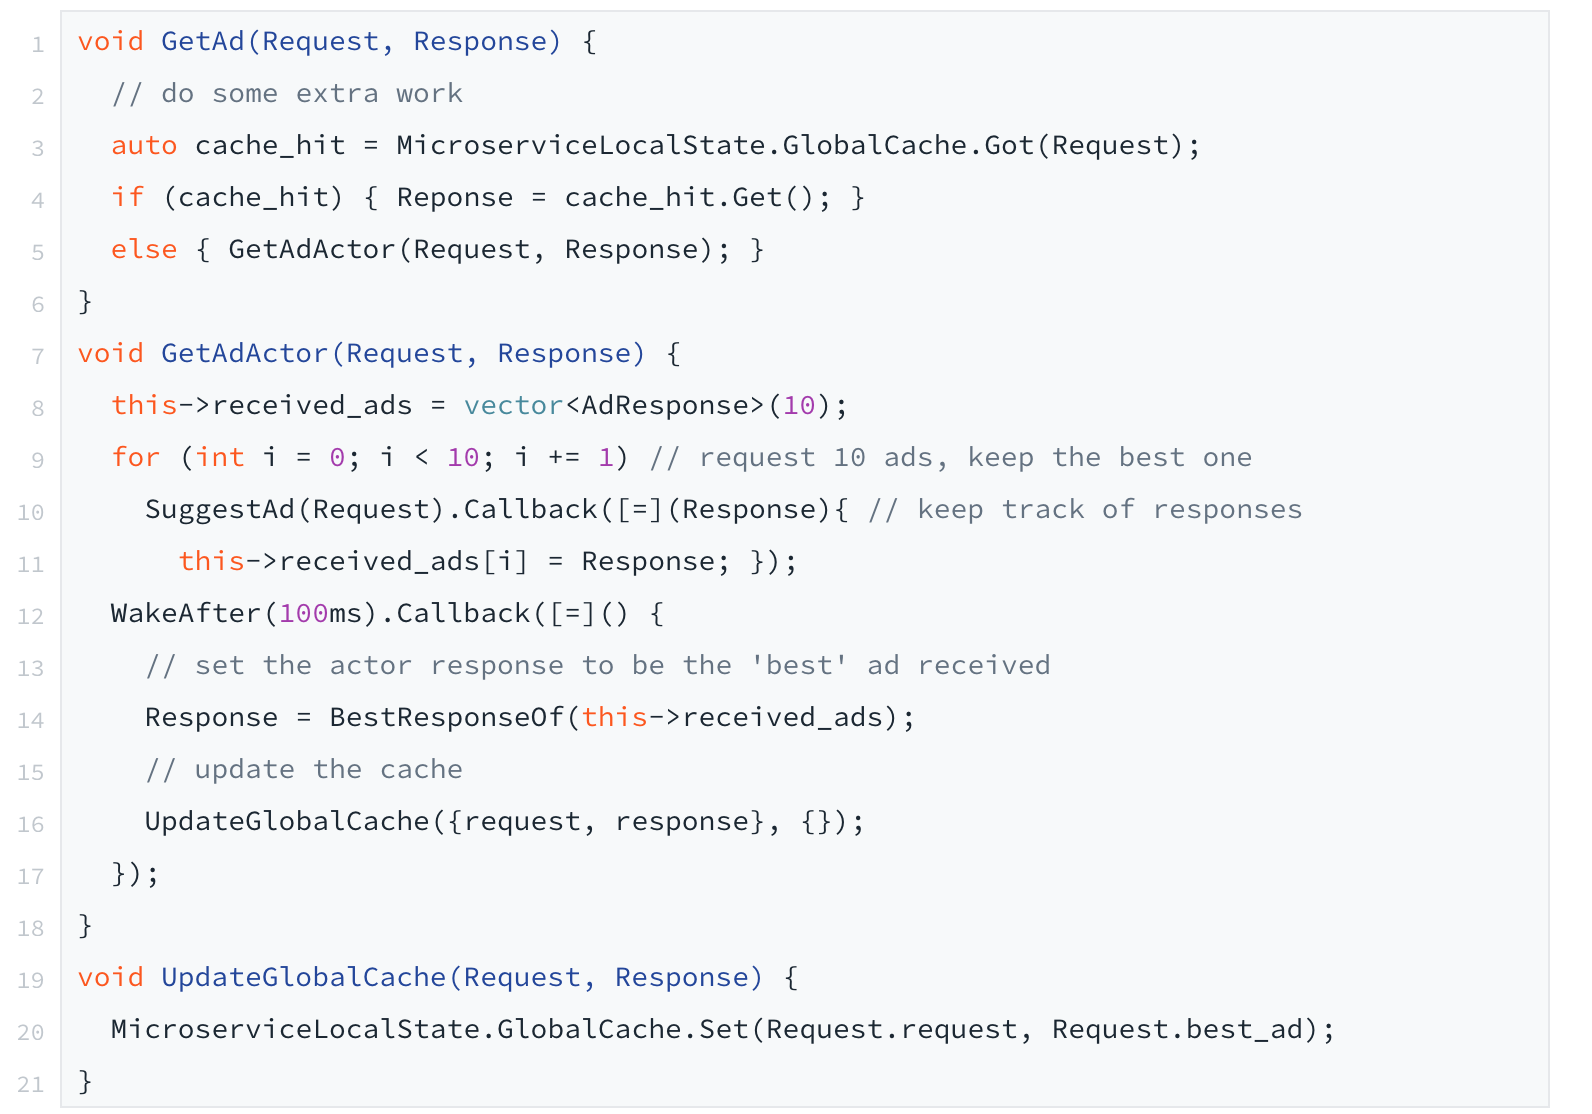
\includegraphics[width=1\linewidth]{content/fig/callbacks.png}
\caption{Callback-based request handler prototype}
\end{figure}

In figure 5.2 we created 2 nanoservices, \code{GetAd} and \code{UpdateGlobalCache}, and 1 actor, \code{GetAdActor}. Since GetInformation forwards the response from another call, we can safely exit the \code{GetAd} nanoservice so it can get to process other requests.
\code{GetAdActor} can have multiple instances of the same state object since it's an actor, and it's reusable and lightweight by design, enabling the existence of multiple such actors at the same time to handle multiple wait-callbacks in parallel. This is enforced by the lifespan of the \code{std::vector received\_ads }. Since the vector is stack-allocated, it'll destroy when the function exits, and if we embed it in the state of the state object, it'll clash with future calls in the case of nanoservices.

While it is possible to implement callbacks nicely with actors or as stateless functions that produce side-effects in nanoservices, we argue that the added complexity does not make this option compelling at the moment, even thou it gives more power to developers.

\subsection*{Choosing the right Future}
Before committing to futures as a means of data sharing, we needed to make sure that this is a viable option, performance-wise. To test these, we created a benchmark environment using the already-implemented mailbox to facilitate the communication between 2 threads, the first one sending a request which will be enqueued in the MPSCQ and retrieved using a promise.
This approach yielded $0.7 \times 10^6$ (a→b a→b a→b) calls/second, drastically affecting the base performance of the MPSCQ, making the standard implementation of futures an infeasible option.

To compensate this, we chose to create a specialized version of the future/promise pair, focusing on raw performance suited for the current use case, allowing the integration of the future/promise inside a pair of request and response, minimizing cache misses. This approach yields $1.8 \times 10^6$ calls/second, being $2.5$ faster than a stantard approach using \code{std::future} 


For the future implementation, we used a heap-allocated \code{BaseFuture} as the central part of the future-promise pair, the actual futures, and promises being similar to a \code{BaseFutureView} with different read or write access, for promises and futures accordingly.
\begin{figure}[H]
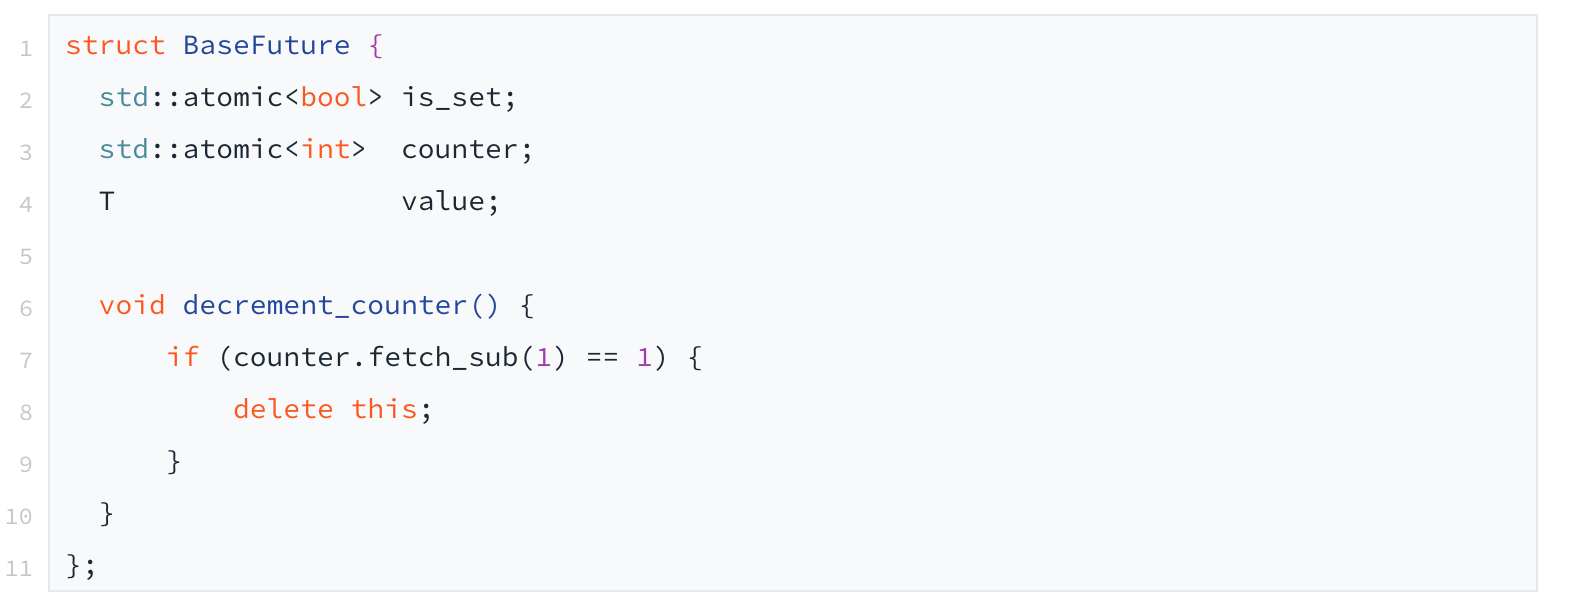
\includegraphics[width=1\linewidth]{content/fig/basefuture.png}
\caption{C++ Future implementation}
\end{figure}

In figure 5.3, we showcase our implementation of the \code{BaseFuture}. The implementation is similar to a shared pointer with a build-in reference counter and a bool flag to simulate a \code{std::optional} field. The code would be further developed to reduce heap-allocations and overhead.


\begin{figure}[H]
\centering
\begin{tikzpicture}[y=.5cm, x=.5cm,font=\sffamily]
 	%axis

	\draw (0,0) -- coordinate (x axis mid) (15,0);
    	\draw (0,0) -- coordinate (y axis mid) (0,15);
    	%ticks
    	\foreach \x in {0, 1, 2.5, 5, 10, 15}
     		\draw (\x,1pt) -- (\x,-3pt)
			node[anchor=north] {\x};
    	\foreach \y in {0,3,...,15}
     		\draw (1pt,\y) -- (-3pt,\y) 
     			node[anchor=east] {\y}; 
	%labels      
	\node[below=0.8cm] at (x axis mid) {$10^6 \times$ number of requests};
	\node[rotate=90, yshift=1.5cm] at (y axis mid) {Time in seconds};

	% plots
	\draw plot[mark=*, mark options={fill=white}] 
		file {future_benchmark.data};
	\draw plot[mark=triangle*, mark options={fill=white} ] 
		file {own_future_benchmark.data};
	\draw plot[mark=square*, mark options={fill=white}]
		file {mpscq_throttled_benchmark.data};
	\draw plot[mark=square*]
		file {pandora_benchmark.data};  
    
	%legend
	\begin{scope}[shift={(4,4)}] 
	\draw[yshift=+3cm, xshift=-1cm] (0,0) -- 
		plot[mark=*, mark options={fill=white}] (0.25,0) -- (0.5,0) 
		node[right]{std future};
	\draw[yshift=\baselineskip+3cm, xshift=-1cm] (0,0) -- 
		plot[mark=triangle*, mark options={fill=white}] (0.25,0) -- (0.5,0)
		node[right]{own future};
	\draw[yshift=2\baselineskip+3cm, xshift=-1cm] (0,0) -- 
		plot[mark=square*, mark options={fill=white}] (0.25,0) -- (0.5,0)
		node[right]{MPSCQ};
	\draw[yshift=3\baselineskip+3cm, xshift=-1cm] (0,0) -- 
		plot[mark=square*, mark options={fill=black}] (0.25,0) -- (0.5,0)
		node[right]{Pandora};
	\end{scope}
\end{tikzpicture}
\caption{Future-Promise Benchmark}
\end{figure}

Figure 5.4 showcases time improvements over the std::promise as well as a throttled version of the first MPSCQ benchmark and a Pandora.cc running example. The benchmark involves a general 2 service application, one of them continually polling the other for information. In the MPSCQ throttled benchmark, the producer can send another request only when the consumer has already processed the request to replicate an exchange of information. The Pandora.cc example is based on 2 simple nanoservices, Multiplication and Addition. The first one wants to compute $X \times 1$ by making $X$ Addition calls to add 1 to the final result, where $X$ is the number of requests on the X-axis.


\section{Designing Nanoservices}
Even thou we started with a set goal, to reduce glue code, we argue that it's better not to enforce strict standards from the beginning. With these in mind, we present a current implementation of a nanoservice, a rather explicit one. Our end-goal and view for this part is going to be explained in chapter 6.1, Future work.

\begin{figure}[H]
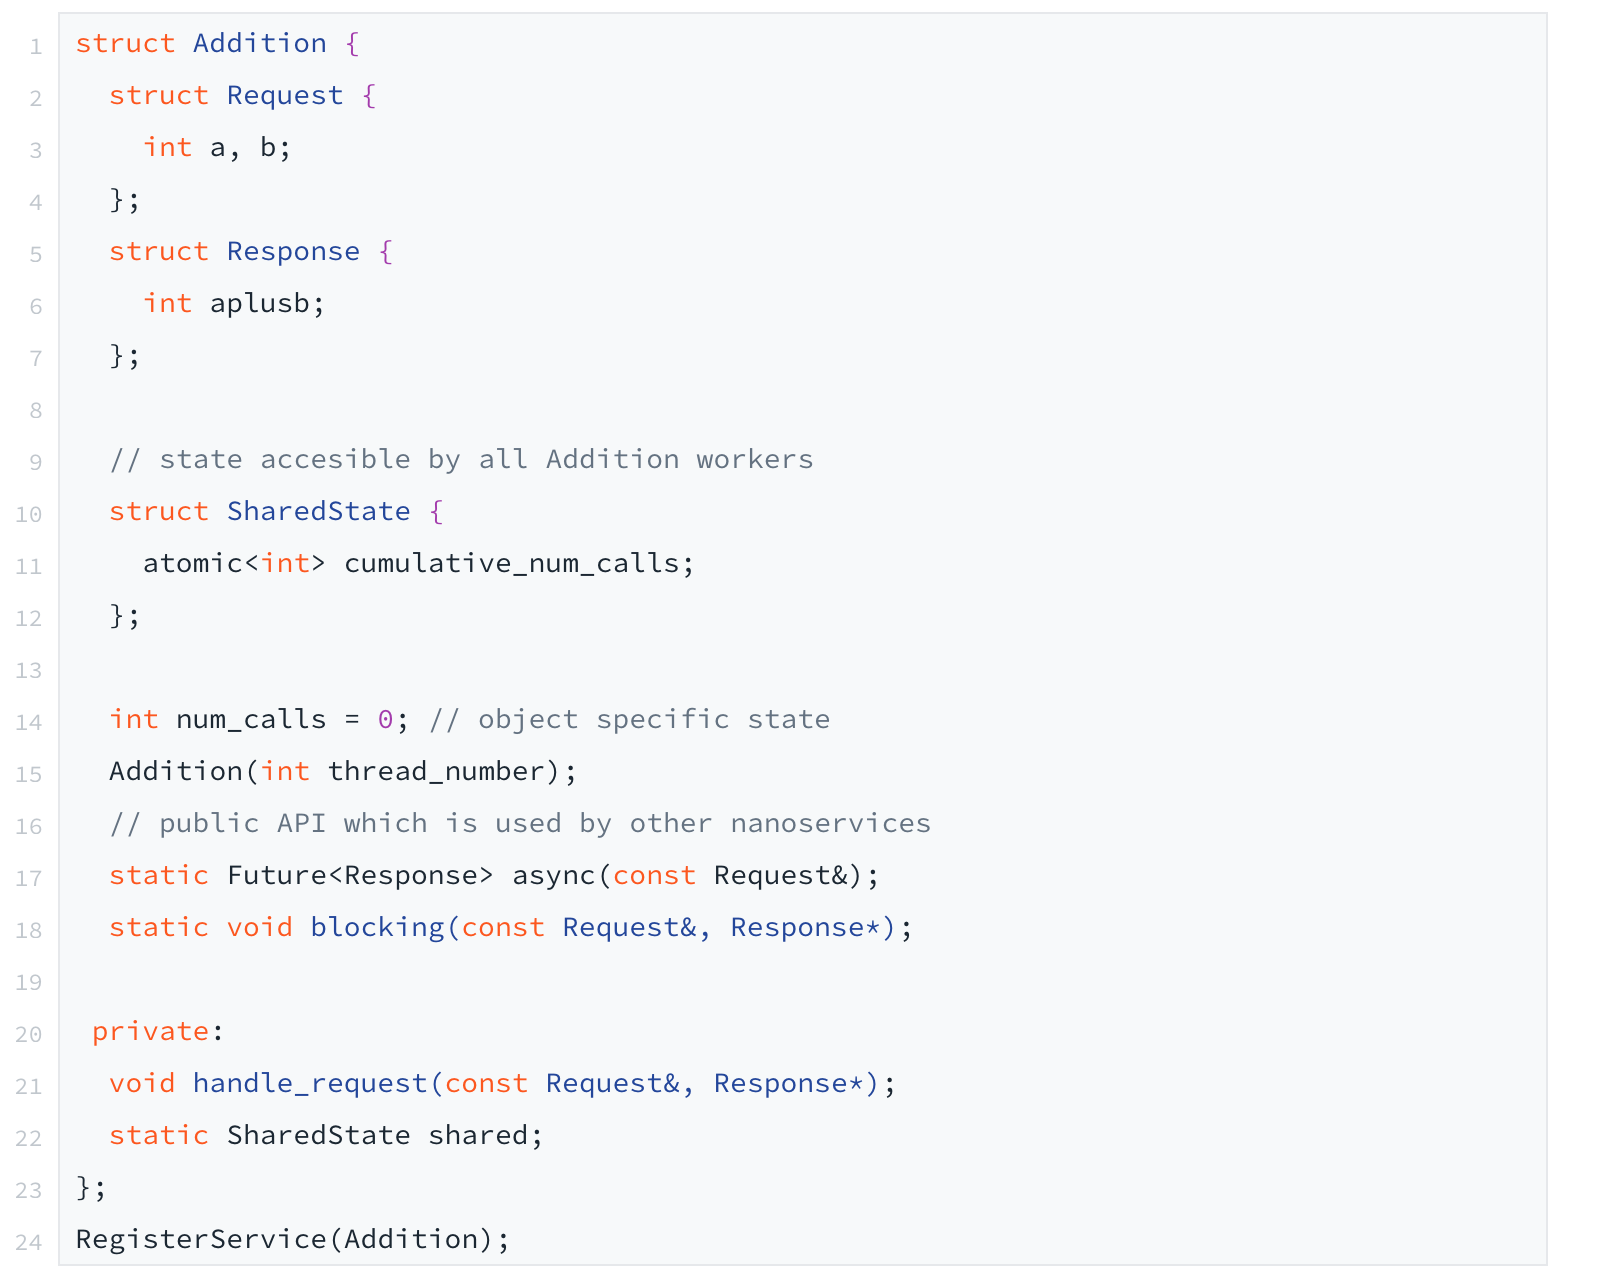
\includegraphics[width=1\linewidth]{content/fig/addition-service.png}
\caption{Nanoserivce demo code}
\end{figure}

In figure 5.5, we present a working \code{Addition} nanoservice. Its purpose is to take 2 numbers and return the sum of those numbers. The code defines the Addition class with the subclasses \code{Request} and \code{Response} accordingly, one constructor, 2 static public API, and one internal handler. Besides all external API's there is one \code{SharedState} class along with a \code{num\_calls} field, enabling the nanoservice to keep a thread-local state. The \code{SharedState} static object allows the individual thread-specific instances to share information if needed. Since this object is shared, the requirement for synchronization mechanisms arrises to implement such cases correctly. The last piece of code is the \code{RegisterService} macro, which enables Pandora.cc to be aware of the presence of the service so it can run the specified services throw the use of the bundling system.
 
Even thou we do not enforce these names in the current iteration of the framework, we'll like to stick by them to check if the current API is sufficient, allowing future changes to be made more quickly if necessary. We opted for this way of writing services since it's somehow similar to other RPC frameworks, users being required to write only the \code{handle\_request} method and the \code{Request} and \code{Response} messages, thus eliminating much necessary glue-code. 

Internally, when performing an async call, the framework look-ups all the possible threads which can run the desired service, and it'll select one, adding the request in that's thread MPSCQ. In the case of blocking calls, the framework checks if the service is configured to execute on this specific thread and calls it as a normal function if that's the case. In case of a failure, it'll throw an exception to signal that. Due to this, it becomes especially tricky to troubleshoot cases where only a subset of threads accept running blocking calls for a specif service.
The option to execute such blocking calls allows users to achieve maximum efficiency without forcing duplicated code.





\section{In depth example overview}
In this section, we want to explain the interactions between various components further analyzing a particular example. The example focuses on a service that recommends internet ads for various sites. Without losing generality, we can assume that we have access to a black-box function, which takes as argument some browser cookies and returns an ad. It's also important to note that we have access to an estimation function, which estimates the likelihood that a user is going to interact with that particular add.

A trivial implementation of this would respond with only one ad, which can yield suboptimal performance. To gain better user interactions, one can generate $X$ ads in parallel and return the best ad based on the estimation function. 

In some cases, the ads can take a while to generate. Instead of waiting for all $X$ ads, the leading service can be configured to wait at most $100ms$ to ensure that the user receives an ad in a decent time, thus not violating the service's SLAs.

A simple Pandora implementation contains a \code{GetAd} nanoservice, which forwards the request to $X$ \code{ProduceAd} nanoservices, waits at most $100ms$ and returns the best ad. The \code{ProduceAd} nanoservice calls the embedded black-box and returns the best ad that is suggested.

Testing the actual performance of the black-box regarding user interactions can be hard to achieve since its hard to deploy different types of black boxes inside a simple service. Using Pandora, each binary could be specified to use a different type of implementation for the \code{ProduceAd} service, which encapsulates the specified black box.

\begin{figure}[H]
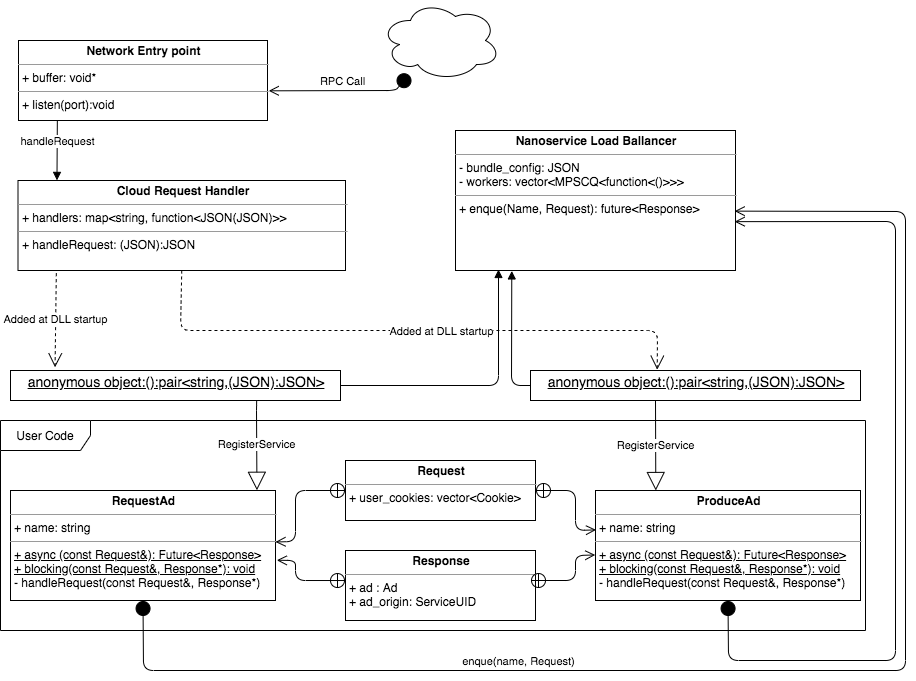
\includegraphics[width=1\linewidth]{content/fig/code-uml.png}
\caption{Ad service complete UML diagram}
\end{figure}

Figure 5.6 described the UML diagram of the entire Pandora binary. It's important to note the usage of the \code{RegisterService} macro. It's run at the load of the nanoservice and it embeds a request handler for that specific service in the \code{CloudRequestHandler}, so it'll be able to handle RPC requests without having to hard-code all handler functions in a big class. Due to this aspect, it's possible to just dinamicly load services directly in the binary, thus reducing the need to recompile the whole project. The relasionship between the nanoservices and the \code{LoadBallencer} is utilised in case of local RPC calls, which don't go over the network.

\begin{figure}[H]
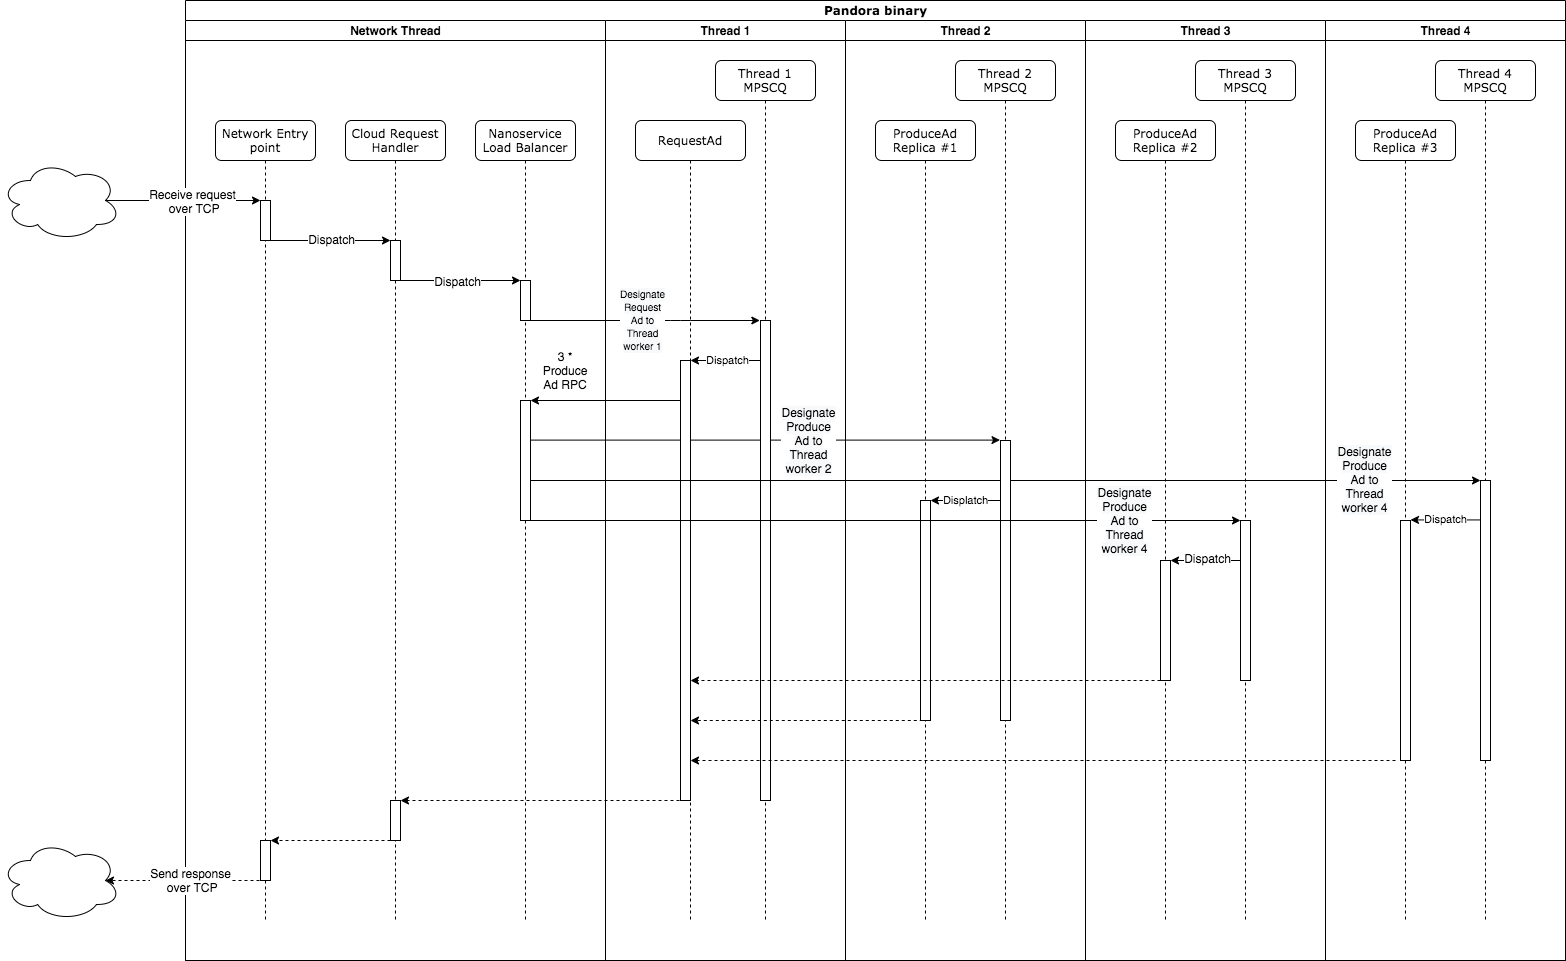
\includegraphics[width=1\linewidth]{content/fig/life-of-a-request.png}
\caption{Life of a request sequence diagram}
\end{figure}

Figure 5.7 showcases a sequence diagram while specifying threads, to furter emphasise the importance of correctly configuring the system. It's important to note that with the current implementation the \code{RequestAd} nanoservice must wait for all 3 \code{ProduceAd} calls to end or to pass 100ms in order to serve another request.


\section{Development process}
As described in chapter 3.1, Motivation, the idea for the framework was a long-planned project.
In the beginning, there was the research, figuring out which technologies are worth taking into consideration and what other developers are using. To facilitate the search for knowledge, GitHub C++ repositories offered much insight into current practices and trends.
The research, shown in chapter 4, paved a long road to success, but it also paved a planned direction and some important end-results as well as some milestones and similar frameworks to keep track of the possibilities. 

Before we started the actual development, the hardest part needed to be dealt with: finding a suitable name. With some inspiration, we settled on Pandora.cc, the first part referencing the classic Greek myth, showcasing Pandora, the first human created on the instructions of Zeus, being gifted by all the gods. 

While all the research provided a compelling direction, we tried to stick to a strict and organized development plan from the beginning, using a streamlined, feature-based approach, which is present in most agile paradigms. The use of the software provided by trello.com and the feature-based approach encouraged an organic growth of the project, offering only essential features while keeping the development process on the road to the end-goal. This pattern is also visible in the structure of this chapter; the mailbox is the first item in the development process, followed by an efficient way to facilitate communication. User-API and the bundle system were refactored numerous times due to code becoming mature. In the end, we introduce a series of other optimizations to facilitate a higher throughput.

Early introduction of examples into the codebase was one of the most critical assets in maintaining a coherent codebase throwout the development period. These examples constitute experiments in the early stages of development, single code endpoints that showcase a use case for a specific library or a header file. With a more refined user-API, the introduction of a hello-world service promoted a broader overview of the library.

\section{Testing}

The early introduction of tests was one of the main targets to look after while developing the framework. While tests may take a while to configure and write, they serve multiple purposes throwout the development process. Ensuring stability is probably one of the first advantages that developers advocate when choosing to test the code in the form of maintaining the correctness of the code. 

While testing comes in a variety of forms and tools, we chose to adhere to a nonconformist way to achieve testing, due to the design and requirements of the project. The fact that one developer did all the development allowed much easier tooling and automatization, cutting out the necessity of stable testing and running environment in the form of a dedicated cloud server. Given this, the execution of all tests before any git-push command is performed using a git-hook. The testing system consists of a python script which executes the experiments and the examples and performs various checks to determine if they satisfy. While this system can be described as simplistic, but we argue that it's a right balance between secure development, maintainability, and initial overhead. In more standard terms, the testing is done using continuous integration, being facilitated by integration tests and performance benchmarks.

Integration tests are primarily used to test big interconnected services or applications. In this particular case, they can be successfully implemented to cover the whole majority of possible code-changes due to the vast logical dependencies of the codebase. This practice takes advantage of the presence of the experiments and examples, covering the entire codebase. To conclude, if the run is accepted or not, the binaries need to produce an expected output that tests their correctness. All the binaries execute 3 times, the first one being the release version, compiled with \code{-std=c++17 -O3} while the second one uses \code{-O1 -fsanitize=address} to check for undefined behavior. The third test involves executing the binaries with \code{valgrind}, yielding a correct execution if there aren't any errors.

Performance benchmarks are not standard, but this fact changes as the application becomes more focused on performance. Subtle changes can affect the overall performance of the application in unsuspected ways, like a change in the task distribution algorithm. Another advantage is that many performance benchmarks offer a history of the performance, making subtle decrements in performance less of a concern to keep track of.

In conclusion, this testing practice offers many advantages to single-developers, being easy to configure and develop while allowing for automated tests so bad-changes do not enter the version control system. The addition of the endpoints (experiments and examples) allows easy testing while developing and a convenient way to achieve continuous integration.